\section{Un exemple complet : de la fenêtre brute aux tokens}\label{sec:exemple}

Les définitions des sections~\ref{sec:unites} et~\ref{sec:ordres} sont plus faciles à saisir sur un cas réel. Nous construisons à la main un motif de 20 événements qui passe par les situations intéressantes :
\begin{itemize}
\item un ordre déjà présent avant la fenêtre ;
\item des ajouts au meilleur prix et plus profond ;
\item des exécutions, dont une qui vide le meilleur niveau ;
\item un odd lot, une taille mixte ;
\item une amélioration de la cote, puis une annulation immédiate ;
\item un même ordre qui change de venue ;
\item un gros ordre lointain.
\end{itemize}
La fenêtre passée au code répète ce motif cinq fois (100 événements, avec des identifiants renouvelés à chaque répétition).

\textbf{Tous les nombres de cette section sont produits par le code du pipeline} (\code{cfm.features}), via le script \code{paper/examples/make\_examples.py}. Ils ne sont pas recopiés à la main.

\subsection{Étape 0 : les événements bruts}
Prix recentrés sur le premier bid, $\tick=0{,}01$ et $\lot=100$ : c'est exactement ce que contient le CSV du challenge.

\begin{table}[H]\centering\scriptsize
\begin{tabular}{rrrcccrrrrcrl}
\toprule
$t$ & venue & order\_id & act. & côté & price & bid & ask & $q^b$ & $q^a$ & trade & flux\\
\midrule
1 & 0 & 5012 & U & B & 0 & 0 & 0{,}01 & 300 & 200 & non & $-$100\\
2 & 1 & 7731 & A & A & 0{,}01 & 0 & 0{,}01 & 300 & 300 & non & 100\\
3 & 1 & 2210 & A & B & $-$0{,}02 & 0 & 0{,}01 & 300 & 300 & non & 200\\
4 & 0 & 7731 & D & A & 0{,}01 & 0 & 0{,}01 & 300 & 200 & oui & $-$100\\
5 & 2 & 9002 & A & A & 0{,}02 & 0 & 0{,}01 & 300 & 200 & non & 37\\
6 & 0 & 5012 & D & B & 0 & 0 & 0{,}01 & 100 & 200 & non & $-$200\\
7 & 3 & 1180 & D & A & 0{,}01 & 0 & 0{,}02 & 100 & 37 & oui & $-$200\\
8 & 1 & 2210 & U & B & $-$0{,}02 & 0 & 0{,}02 & 100 & 37 & non & 100\\
9 & 2 & 4040 & A & A & 0{,}01 & 0 & 0{,}01 & 100 & 100 & non & 100\\
10 & 2 & 4040 & D & A & 0{,}01 & 0 & 0{,}02 & 100 & 37 & non & $-$100\\
11 & 0 & 3333 & A & B & 0{,}01 & 0{,}01 & 0{,}02 & 150 & 37 & non & 150\\
12 & 4 & 9002 & U & A & 0{,}02 & 0{,}01 & 0{,}02 & 150 & 100 & non & 63\\
13 & 4 & 3333 & D & B & 0{,}01 & 0 & 0{,}02 & 100 & 100 & oui & $-$150\\
14 & 5 & 8888 & A & B & $-$0{,}06 & 0 & 0{,}02 & 100 & 100 & non & 1000\\
15 & 5 & 8888 & U & B & $-$0{,}06 & 0 & 0{,}02 & 100 & 100 & non & $-$500\\
16 & 0 & 1212 & A & A & 0{,}02 & 0 & 0{,}02 & 100 & 200 & non & 100\\
17 & 0 & 1212 & U & A & 0{,}02 & 0 & 0{,}02 & 100 & 300 & non & 100\\
18 & 3 & 1212 & D & A & 0{,}02 & 0 & 0{,}03 & 100 & 400 & oui & $-$300\\
19 & 1 & 7070 & A & A & 0{,}02 & 0 & 0{,}02 & 100 & 100 & non & 100\\
20 & 1 & 2210 & D & B & $-$0{,}02 & 0 & 0{,}02 & 100 & 100 & non & $-$300\\
\bottomrule
\end{tabular}
\caption{Le motif brut. B = côté acheteur (bid), A = côté vendeur (ask). Les colonnes bid, ask, $q^b$ et $q^a$ décrivent le carnet agrégé \emph{après} l'événement.}
\label{tab:exraw}
\end{table}

\begin{figure}[H]\centering
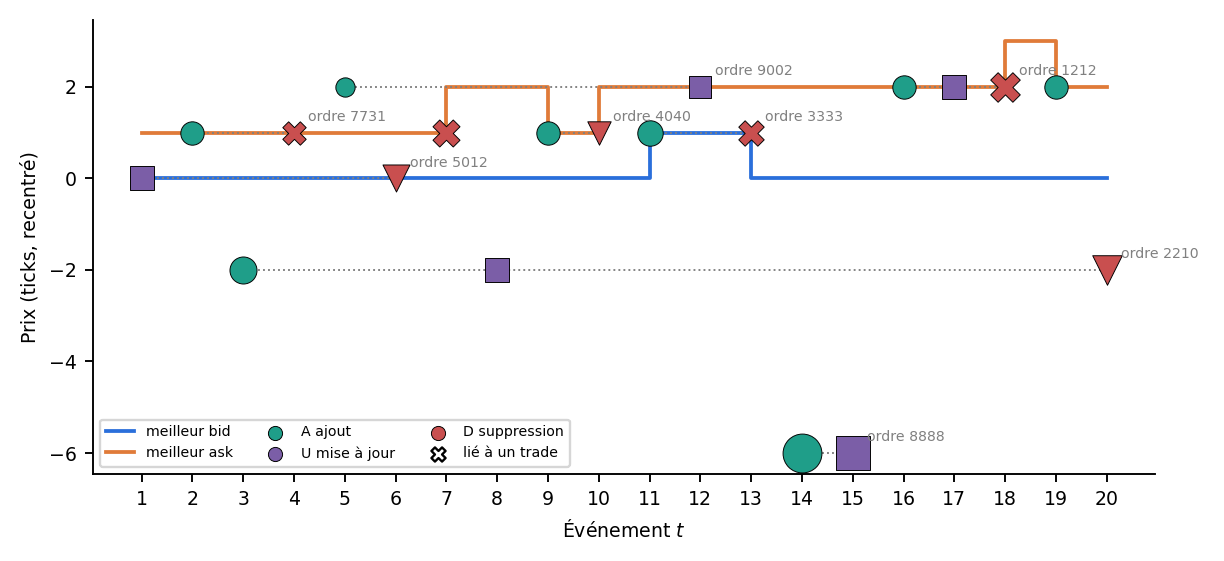
\includegraphics[width=\linewidth]{figures/ex_motif.png}
\caption{Le motif en image. Les escaliers sont les meilleures limites ; chaque marqueur est un événement (couleur = action, croix = lié à un trade, taille $\propto\sqrt{|f|}$). Les pointillés relient les événements d'un \emph{même ordre} : ce sont les parcours que les tokens d'occurrence et d'action précédente encodent.}
\label{fig:exmotif}
\end{figure}

\subsection{Étape 1 : l'identité des ordres}
Les identifiants bruts (5012, 7731, \dots) sont remplacés par leur rang de première apparition $\rho_t$ (section~\ref{sec:donnees}). Seules les égalités comptent : 5012 devient 0, 7731 devient 1, 2210 devient 2, etc. On en déduit l'occurrence $n_t$, l'action précédente du même ordre $a^{\leftarrow}_t$ et l'écart $g_t$ (tableau~\ref{tab:exderived}). Trois parcours se lisent directement :

\begin{itemize}
\item \textbf{L'ordre 2210} ($\rho=2$) apparaît à $t=3$ (ajout), $t=8$ (mise à jour) et $t=20$ (suppression). On obtient $n=(0,1,2)$, $a^{\leftarrow}=(\text{—},A,U)$ et $g=(0,5,12)$.
\item \textbf{L'ordre 5012} ($\rho=0$) apparaît d'abord sous forme d'une \emph{mise à jour}. Il existait donc avant la fenêtre : la troncature est visible. Dans le bloc \code{orders}, il compte dans \code{first\_seen\_U}.
\item \textbf{L'ordre 1212} ($\rho=8$) est ajouté puis modifié sur la venue 0, puis exécuté sur la venue 3 ($t=18$). C'est une répétition « inter-venue », possible parce que le carnet est agrégé (\code{cross\_venue\_repeat}).
\end{itemize}

\subsection{Étape 2 : passer en unités naturelles}
\begin{table}[H]\centering\scriptsize
\begin{tabular}{rrrrrrrrrl}
\toprule
$t$ & $\rho_t$ & $n_t$ & $a^{\leftarrow}_t$ & $g_t$ & $S_t$ & $h_t$ & $D_t$ & $F_t$ & lecture\\
\midrule
1 & 0 & 0 & — & 0 & 1 & 0 & 0 & $-$1 & \parbox[t]{6.2cm}{\raggedright\scriptsize ordre déjà présent avant la fenêtre (1re apparition = U), réduit d'un lot}\\
2 & 1 & 0 & — & 0 & 1 & 0 & 0 & 1 & \parbox[t]{6.2cm}{\raggedright\scriptsize ajout d'un lot au meilleur ask}\\
3 & 2 & 0 & — & 0 & 1 & 0 & 2 & 2 & \parbox[t]{6.2cm}{\raggedright\scriptsize ajout de 2 lots, 2 ticks derrière le meilleur bid}\\
4 & 1 & 1 & A & 2 & 1 & 0 & 0 & $-$1 & \parbox[t]{6.2cm}{\raggedright\scriptsize l'ordre de t=2 est exécuté (suppression liée à un trade)}\\
5 & 3 & 0 & — & 0 & 1 & 0 & 1 & 0{,}37 & \parbox[t]{6.2cm}{\raggedright\scriptsize odd lot (37 actions), 1 tick derrière le meilleur ask}\\
6 & 0 & 1 & U & 5 & 1 & 0 & 0 & $-$2 & \parbox[t]{6.2cm}{\raggedright\scriptsize annulation de l'ordre pré-existant}\\
7 & 4 & 0 & — & 0 & 2 & 1 & $-$1 & $-$2 & \parbox[t]{6.2cm}{\raggedright\scriptsize trade vide le meilleur ask : l'ask passe à 0,02, spread 2 ticks, le mid monte d'un demi-tick}\\
8 & 2 & 1 & A & 5 & 2 & 0 & 2 & 1 & \parbox[t]{6.2cm}{\raggedright\scriptsize l'ordre profond de t=3 grossit d'un lot}\\
9 & 5 & 0 & — & 0 & 1 & $-$1 & 0 & 1 & \parbox[t]{6.2cm}{\raggedright\scriptsize ajout DANS le spread : améliore l'ask}\\
10 & 5 & 1 & A & 1 & 2 & 1 & $-$1 & $-$1 & \parbox[t]{6.2cm}{\raggedright\scriptsize le même ordre est annulé aussitôt (ajouté puis supprimé)}\\
11 & 6 & 0 & — & 0 & 1 & 1 & 0 & 1{,}5 & \parbox[t]{6.2cm}{\raggedright\scriptsize ajout DANS le spread côté bid, taille mixte (1,5 lot)}\\
12 & 3 & 1 & A & 7 & 1 & 0 & 0 & 0{,}63 & \parbox[t]{6.2cm}{\raggedright\scriptsize l'odd lot de t=5 est complété à un lot rond}\\
13 & 6 & 1 & A & 2 & 2 & $-$1 & $-$1 & $-$1{,}5 & \parbox[t]{6.2cm}{\raggedright\scriptsize l'ordre de t=11 est exécuté : le bid redescend}\\
14 & 7 & 0 & — & 0 & 2 & 0 & 6 & 10 & \parbox[t]{6.2cm}{\raggedright\scriptsize gros ordre (10 lots) très loin (6 ticks)}\\
15 & 7 & 1 & A & 1 & 2 & 0 & 6 & $-$5 & \parbox[t]{6.2cm}{\raggedright\scriptsize réduit de moitié}\\
16 & 8 & 0 & — & 0 & 2 & 0 & 0 & 1 & \parbox[t]{6.2cm}{\raggedright\scriptsize ajout d'un lot au meilleur ask}\\
17 & 8 & 1 & A & 1 & 2 & 0 & 0 & 1 & \parbox[t]{6.2cm}{\raggedright\scriptsize le même ordre grossit}\\
18 & 8 & 2 & U & 1 & 3 & 1 & $-$1 & $-$3 & \parbox[t]{6.2cm}{\raggedright\scriptsize exécuté sur une AUTRE venue (3) : l'ask passe à 0,03, spread 3 ticks}\\
19 & 9 & 0 & — & 0 & 2 & $-$1 & 0 & 1 & \parbox[t]{6.2cm}{\raggedright\scriptsize ajout dans le spread, l'ask revient à 0,02}\\
20 & 2 & 2 & U & 12 & 2 & 0 & 2 & $-$3 & \parbox[t]{6.2cm}{\raggedright\scriptsize annulation de l'ordre profond de t=3}\\
\bottomrule
\end{tabular}
\caption{Grandeurs dérivées, calculées par \code{features/common.py} : spread $S_t$ en ticks, variation du mid $h_t$ en demi-ticks, distance au meilleur prix de son côté $D_t$ en ticks, flux $F_t$ en lots.}
\label{tab:exderived}
\end{table}

\paragraph{Quatre calculs détaillés.}
\begin{itemize}
\item \textbf{$t=5$} (odd lot, côté ask, prix $0{,}02$, ask après l'événement $0{,}01$) :
$D_5=(p_5-\alpha_5)/\tick=(0{,}02-0{,}01)/0{,}01=1$, soit un tick derrière le meilleur ask ; $F_5=37/100=0{,}37<1$, donc un odd lot.
\item \textbf{$t=7$} (un trade vide le meilleur ask) : l'ask passe de $0{,}01$ à $0{,}02$, donc $S_7=2$. Le mid passe de $0{,}005$ à $0{,}010$, donc $h_7=2\times0{,}005/0{,}01=1$ : une hausse d'un demi-tick.
\item \textbf{$t=11$} (ajout côté bid à $0{,}01$, qui améliore le bid) : après l'événement, $b_{11}=0{,}01$, donc $D_{11}=(b_{11}-p_{11})/\tick=0$, et $F_{11}=1{,}5$, une taille mixte.
\item \textbf{$t=14$} (gros ordre lointain) : $D_{14}=(0-(-0{,}06))/0{,}01=6$ et $F_{14}=10$ lots.
\end{itemize}

\subsection{Étape 3 : discrétiser en tokens}
Chaque grandeur passe par une fonction de bucket à seuils fixés, $B(x;c)=1+\#\{j:c_j\le x\}$ (0 si $x$ n'est pas défini).

Pour la taille, les seuils sont $c=(10^{-9},\,1-10^{-9},\,1+10^{-9},\,2+10^{-9},\,5+10^{-9},\,10+10^{-9})$ :
\begin{align*}
t=5:&\quad B(0{,}37;c)=1+\#\{10^{-9}\}=2\ \Rightarrow\ \text{« odd »},\\
t=1:&\quad B(1;c)=1+\#\{10^{-9},\,1-10^{-9}\}=3\ \Rightarrow\ \text{« = 1 lot »},\\
t=14:&\quad B(10;c)=1+5=6\ \Rightarrow\ \text{« (5,10] »}.
\end{align*}
Les deux seuils $1\pm10^{-9}$ isolent exactement « un lot rond », qui est la taille la plus fréquente sur ce marché.

\begin{table}[H]\centering\scriptsize\setlength{\tabcolsep}{2.5pt}
\begin{tabular}{rccccccccccc}
\toprule
$t$ & act & côté & trade & venue & pos & taille & spread & Δmid & occ & préc. & signe\\
\midrule
1 & 3\,{\tiny(U)} & 2\,{\tiny(bid)} & 1\,{\tiny(non)} & 1\,{\tiny(v0)} & 2\,{\tiny(=)} & 3\,{\tiny(=1 lot)} & 2\,{\tiny(1)} & 3\,{\tiny(0)} & 1\,{\tiny(1re)} & 0\,{\tiny(aucune)} & 1\,{\tiny(<0)}\\
2 & 1\,{\tiny(A)} & 1\,{\tiny(ask)} & 1\,{\tiny(non)} & 2\,{\tiny(v1)} & 2\,{\tiny(=)} & 3\,{\tiny(=1 lot)} & 2\,{\tiny(1)} & 3\,{\tiny(0)} & 1\,{\tiny(1re)} & 0\,{\tiny(aucune)} & 3\,{\tiny(>0)}\\
3 & 1\,{\tiny(A)} & 2\,{\tiny(bid)} & 1\,{\tiny(non)} & 2\,{\tiny(v1)} & 4\,{\tiny(+2)} & 4\,{\tiny((1,2])} & 2\,{\tiny(1)} & 3\,{\tiny(0)} & 1\,{\tiny(1re)} & 0\,{\tiny(aucune)} & 3\,{\tiny(>0)}\\
4 & 2\,{\tiny(D)} & 1\,{\tiny(ask)} & 2\,{\tiny(oui)} & 1\,{\tiny(v0)} & 2\,{\tiny(=)} & 3\,{\tiny(=1 lot)} & 2\,{\tiny(1)} & 3\,{\tiny(0)} & 2\,{\tiny(2e)} & 1\,{\tiny(A)} & 1\,{\tiny(<0)}\\
5 & 1\,{\tiny(A)} & 1\,{\tiny(ask)} & 1\,{\tiny(non)} & 3\,{\tiny(v2)} & 3\,{\tiny(+1)} & 2\,{\tiny(odd)} & 2\,{\tiny(1)} & 3\,{\tiny(0)} & 1\,{\tiny(1re)} & 0\,{\tiny(aucune)} & 3\,{\tiny(>0)}\\
6 & 2\,{\tiny(D)} & 2\,{\tiny(bid)} & 1\,{\tiny(non)} & 1\,{\tiny(v0)} & 2\,{\tiny(=)} & 4\,{\tiny((1,2])} & 2\,{\tiny(1)} & 3\,{\tiny(0)} & 2\,{\tiny(2e)} & 3\,{\tiny(U)} & 1\,{\tiny(<0)}\\
7 & 2\,{\tiny(D)} & 1\,{\tiny(ask)} & 2\,{\tiny(oui)} & 4\,{\tiny(v3)} & 1\,{\tiny(in)} & 4\,{\tiny((1,2])} & 3\,{\tiny(2)} & 4\,{\tiny(hausse)} & 1\,{\tiny(1re)} & 0\,{\tiny(aucune)} & 1\,{\tiny(<0)}\\
8 & 3\,{\tiny(U)} & 2\,{\tiny(bid)} & 1\,{\tiny(non)} & 2\,{\tiny(v1)} & 4\,{\tiny(+2)} & 3\,{\tiny(=1 lot)} & 3\,{\tiny(2)} & 3\,{\tiny(0)} & 2\,{\tiny(2e)} & 1\,{\tiny(A)} & 3\,{\tiny(>0)}\\
9 & 1\,{\tiny(A)} & 1\,{\tiny(ask)} & 1\,{\tiny(non)} & 3\,{\tiny(v2)} & 2\,{\tiny(=)} & 3\,{\tiny(=1 lot)} & 2\,{\tiny(1)} & 2\,{\tiny(baisse)} & 1\,{\tiny(1re)} & 0\,{\tiny(aucune)} & 3\,{\tiny(>0)}\\
10 & 2\,{\tiny(D)} & 1\,{\tiny(ask)} & 1\,{\tiny(non)} & 3\,{\tiny(v2)} & 1\,{\tiny(in)} & 3\,{\tiny(=1 lot)} & 3\,{\tiny(2)} & 4\,{\tiny(hausse)} & 2\,{\tiny(2e)} & 1\,{\tiny(A)} & 1\,{\tiny(<0)}\\
11 & 1\,{\tiny(A)} & 2\,{\tiny(bid)} & 1\,{\tiny(non)} & 1\,{\tiny(v0)} & 2\,{\tiny(=)} & 4\,{\tiny((1,2])} & 2\,{\tiny(1)} & 4\,{\tiny(hausse)} & 1\,{\tiny(1re)} & 0\,{\tiny(aucune)} & 3\,{\tiny(>0)}\\
12 & 3\,{\tiny(U)} & 1\,{\tiny(ask)} & 1\,{\tiny(non)} & 5\,{\tiny(v4)} & 2\,{\tiny(=)} & 2\,{\tiny(odd)} & 2\,{\tiny(1)} & 3\,{\tiny(0)} & 2\,{\tiny(2e)} & 1\,{\tiny(A)} & 3\,{\tiny(>0)}\\
13 & 2\,{\tiny(D)} & 2\,{\tiny(bid)} & 2\,{\tiny(oui)} & 5\,{\tiny(v4)} & 1\,{\tiny(in)} & 4\,{\tiny((1,2])} & 3\,{\tiny(2)} & 2\,{\tiny(baisse)} & 2\,{\tiny(2e)} & 1\,{\tiny(A)} & 1\,{\tiny(<0)}\\
14 & 1\,{\tiny(A)} & 2\,{\tiny(bid)} & 1\,{\tiny(non)} & 6\,{\tiny(v5)} & 6\,{\tiny(>+5)} & 6\,{\tiny((5,10])} & 3\,{\tiny(2)} & 3\,{\tiny(0)} & 1\,{\tiny(1re)} & 0\,{\tiny(aucune)} & 3\,{\tiny(>0)}\\
15 & 3\,{\tiny(U)} & 2\,{\tiny(bid)} & 1\,{\tiny(non)} & 6\,{\tiny(v5)} & 6\,{\tiny(>+5)} & 5\,{\tiny((2,5])} & 3\,{\tiny(2)} & 3\,{\tiny(0)} & 2\,{\tiny(2e)} & 1\,{\tiny(A)} & 1\,{\tiny(<0)}\\
16 & 1\,{\tiny(A)} & 1\,{\tiny(ask)} & 1\,{\tiny(non)} & 1\,{\tiny(v0)} & 2\,{\tiny(=)} & 3\,{\tiny(=1 lot)} & 3\,{\tiny(2)} & 3\,{\tiny(0)} & 1\,{\tiny(1re)} & 0\,{\tiny(aucune)} & 3\,{\tiny(>0)}\\
17 & 3\,{\tiny(U)} & 1\,{\tiny(ask)} & 1\,{\tiny(non)} & 1\,{\tiny(v0)} & 2\,{\tiny(=)} & 3\,{\tiny(=1 lot)} & 3\,{\tiny(2)} & 3\,{\tiny(0)} & 2\,{\tiny(2e)} & 1\,{\tiny(A)} & 3\,{\tiny(>0)}\\
18 & 2\,{\tiny(D)} & 1\,{\tiny(ask)} & 2\,{\tiny(oui)} & 4\,{\tiny(v3)} & 1\,{\tiny(in)} & 5\,{\tiny((2,5])} & 4\,{\tiny(3–4)} & 4\,{\tiny(hausse)} & 3\,{\tiny(3e)} & 3\,{\tiny(U)} & 1\,{\tiny(<0)}\\
19 & 1\,{\tiny(A)} & 1\,{\tiny(ask)} & 1\,{\tiny(non)} & 2\,{\tiny(v1)} & 2\,{\tiny(=)} & 3\,{\tiny(=1 lot)} & 3\,{\tiny(2)} & 2\,{\tiny(baisse)} & 1\,{\tiny(1re)} & 0\,{\tiny(aucune)} & 3\,{\tiny(>0)}\\
20 & 2\,{\tiny(D)} & 2\,{\tiny(bid)} & 1\,{\tiny(non)} & 2\,{\tiny(v1)} & 4\,{\tiny(+2)} & 5\,{\tiny((2,5])} & 3\,{\tiny(2)} & 3\,{\tiny(0)} & 3\,{\tiny(3e)} & 3\,{\tiny(U)} & 1\,{\tiny(<0)}\\
\bottomrule
\end{tabular}
\caption{Les onze tokens de chaque événement : l'indice d'abord, la signification entre parenthèses. Pour \code{pos}, « in » signifie « dans le spread », « = » « au meilleur » et « $+k$ » « $k$ ticks derrière ».}
\label{tab:extokens}
\end{table}

\begin{figure}[H]\centering
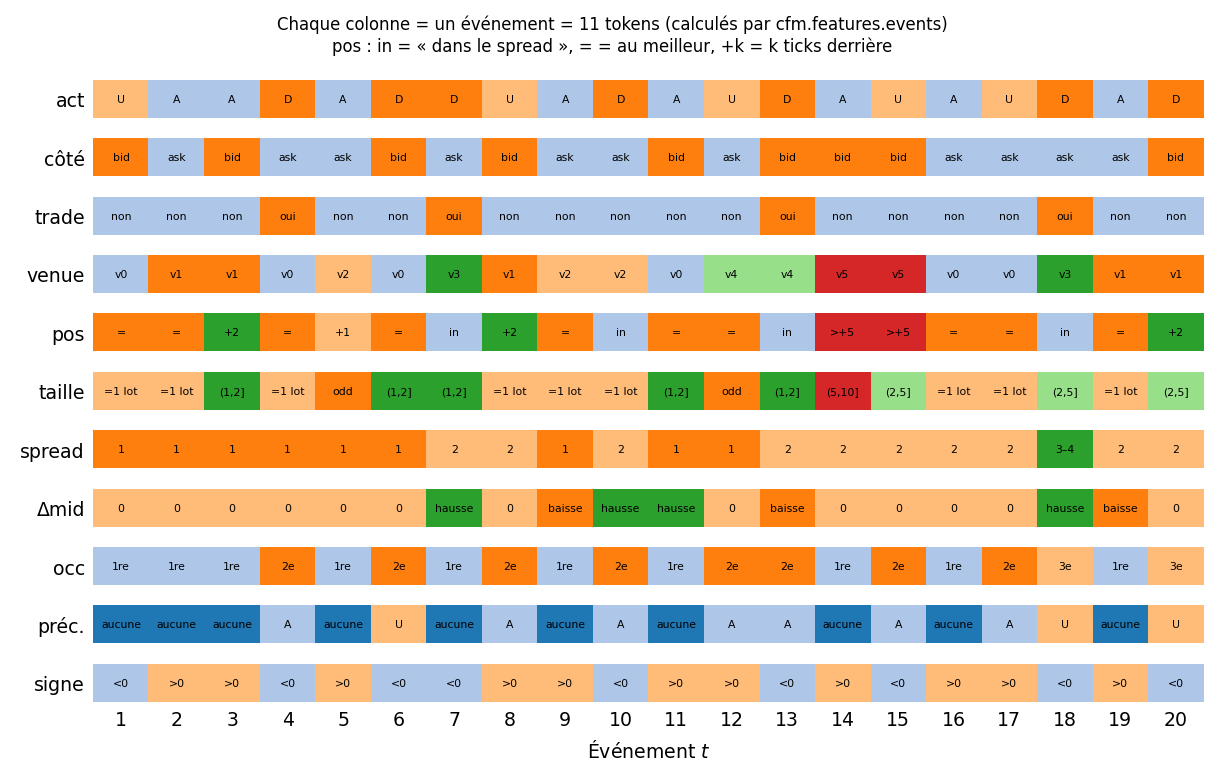
\includegraphics[width=\linewidth]{figures/ex_tokens.png}
\caption{La même information en bandeau : une colonne par événement, une ligne par token. C'est littéralement ce que voit SignatureNet avant ses couches d'embedding.}
\label{fig:extokens}
\end{figure}

\subsection{Ce que l'exemple révèle : $D_t$ est mesuré \emph{après} l'événement}\label{sec:dpost}
L'exemple met au jour une subtilité de la définition. Elle n'apparaît pas à la lecture des formules.

\begin{itemize}
\item \textbf{Ajouts qui améliorent la cote ($t=9$, $t=11$).} L'ordre devient lui-même le meilleur prix. Il est donc codé « = » (au meilleur), et non « in » (dans le spread).
\item \textbf{Suppressions qui vident le meilleur niveau ($t=7,10,13,18$).} Après l'événement, la meilleure limite a reculé, et le prix de l'ordre supprimé se retrouve \emph{à l'intérieur} du nouveau spread : $D_t=-1$, codé « in ».
\end{itemize}

Dans le pipeline actuel, le token « in » signifie donc en pratique « \emph{cet événement a vidé le meilleur niveau} ». C'est une information utile, que le modèle a exploitée telle quelle (LB $0{,}6351$), mais son nom est trompeur. La correction naturelle consiste à mesurer la position par rapport au carnet \emph{avant} l'événement :
\begin{equation}
D^{\text{pré}}_t=\frac1\tick\begin{cases}b_{t-1}-p_t&s_t=B,\\ p_t-\alpha_{t-1}&s_t=A.\end{cases}
\end{equation}
Avec cette définition, $D^{\text{pré}}_9=(0{,}01-0{,}02)/0{,}01=-1$ (amélioration de la cote : « in »), et $D^{\text{pré}}_7=(0{,}01-0{,}01)/0{,}01=0$ (suppression au meilleur : « = »).

Les deux versions portent des informations différentes. Garder les deux tokens (« où était l'ordre » et « ce que l'événement a fait au carnet ») est une expérience prévue pour la V5. Elle n'a pas encore été mesurée.

\subsection{Étape 4 : des tokens au vecteur d'entrée}
L'événement $t=5$ a les indices de tokens $(1,1,1,3,3,2,2,3,1,0,3)$ (tableau~\ref{tab:extokens}). Son vecteur d'entrée est
\begin{multline}
x^{(0)}_5=\LN\big(P_5+E_{\text{act}}[1]+E_{\text{côté}}[1]+E_{\text{trade}}[1]+E_{\text{venue}}[3]+E_{\text{pos}}[3]+E_{\text{taille}}[2]\\
+E_{\text{spread}}[2]+E_{\Delta\text{mid}}[3]+E_{\text{occ}}[1]+E_{\text{préc}}[0]+E_{\text{signe}}[3]+W_{\text{in}}c_5+b_{\text{in}}\big),
\end{multline}
une somme de 11 vecteurs appris de dimension 96, plus la projection des canaux continus. Deux odd lots placés 1 tick derrière l'ask partagent ainsi $E_{\text{pos}}[3]+E_{\text{taille}}[2]$, quel que soit le titre. Ce sont les couches suivantes (convolutions, attention) qui apprennent que leur \emph{fréquence} et leur \emph{enchaînement} diffèrent d'un titre à l'autre.

\subsection{Étape 5 : les statistiques de la fenêtre}
Sur la fenêtre de 100 événements (le motif répété), les blocs de la section~\ref{sec:blocs} valent :
\begin{table}[H]\centering\small
\begin{tabular}{lll}
\toprule
Bloc & Colonne & Valeur\\
\midrule
\code{ticks} & \code{spread\_1} & 0{,}45\\
\code{ticks} & \code{spread\_2} & 0{,}5\\
\code{ticks} & \code{spread\_3\_4} & 0{,}05\\
\code{ticks} & \code{mid\_move} & 0{,}39\\
\code{ticks} & \code{move\_half\_tick} & 1\\
\addlinespace
\code{lots} & \code{flux\_round} & 0{,}8\\
\code{lots} & \code{flux\_odd} & 0{,}1\\
\code{lots} & \code{flux\_mixed} & 0{,}1\\
\code{lots} & \code{flux\_exactly\_1lot} & 0{,}45\\
\code{lots} & \code{flux\_ge\_10lots} & 0{,}05\\
\addlinespace
\code{position} & \code{pos\_inside} & 0{,}2\\
\code{position} & \code{pos\_best} & 0{,}5\\
\code{position} & \code{pos\_d1} & 0{,}05\\
\code{position} & \code{pos\_d2} & 0{,}15\\
\code{position} & \code{pos\_d6p} & 0{,}1\\
\addlinespace
\code{orders} & \code{orders\_per\_event} & 0{,}5\\
\code{orders} & \code{repeat\_share} & 0{,}5\\
\code{orders} & \code{first\_seen\_U} & 0{,}1\\
\code{orders} & \code{A\_to\_D} & 0{,}3\\
\code{orders} & \code{D\_trade\_share} & 0{,}571\\
\code{orders} & \code{cross\_venue\_repeat} & 0{,}4\\
\addlinespace
\bottomrule
\end{tabular}
\caption{Extrait des blocs de fenêtre, calculés par \code{features/window.py}.}
\label{tab:exblocks}
\end{table}
\noindent Chaque valeur se vérifie sur le motif :
\begin{itemize}
\item \code{flux\_round} $=0{,}8$ : 16 événements sur 20 ont un flux multiple entier d'un lot. Les exceptions sont $t=5,12$ (odd) et $t=11,13$ (mixtes).
\item \code{pos\_inside} $=0{,}2$ : exactement les 4 suppressions qui vident le meilleur niveau (section~\ref{sec:dpost}).
\item \code{first\_seen\_U} $=0{,}1$ : 1 ordre sur les 10 du motif (5012) apparaît d'abord en mise à jour.
\item \code{A\_to\_D} $=0{,}3$ : parmi les 10 répétitions, 3 passent d'un ajout à une suppression ($t=4,10,13$).
\item \code{D\_trade\_share} $=4/7$ : 4 des 7 suppressions sont des exécutions ($t=4,7,13,18$).
\item \code{cross\_venue\_repeat} $=0{,}4$ : 4 des 10 répétitions changent de venue ($t=4,12,13,18$).
\item \code{move\_half\_tick} $=1$ : tous les mouvements du mid font exactement un demi-tick.
\end{itemize}

\subsection{Pourquoi pas une normalisation relative : un contre-exemple chiffré}
Deux fenêtres identiques en tout, sauf le spread : constant à 1 tick dans l'une, à 5 ticks dans l'autre. Ce sont typiquement un titre à gros tick et un titre à petit tick.
\begin{table}[H]\centering\small
\begin{tabular}{llcc}
\toprule
Représentation & Colonne & spread 1 tick & spread 5 ticks\\
\midrule
avant (relative) & \code{spread\_rel\_mean} & 0{,}693 & 0{,}693\\
avant (relative) & \code{spread\_rel\_std} & 0 & 0\\
avant (relative) & \code{price\_pos\_rel\_mean} & 0 & 0\\
\midrule
maintenant (ticks) & \code{spread\_1} & 1 & 0\\
maintenant (ticks) & \code{spread\_5p} & 0 & 1\\
maintenant (ticks) & \code{spread\_t\_median} & 1 & 5\\
\bottomrule
\end{tabular}
\caption{L'ancienne représentation (relative à la médiane locale) ne distingue pas les deux fenêtres (Proposition~\ref{prop:scale}). Les colonnes en ticks les séparent sans ambiguïté.}
\label{tab:exscale}
\end{table}
